
%(BEGIN_QUESTION)
% Copyright 2008, Tony R. Kuphaldt, released under the Creative Commons Attribution License (v 1.0)
% This means you may do almost anything with this work of mine, so long as you give me proper credit

Estimate the slope of a parabola ($y = x^2$) at $x=2$ by calculating the slope of successive secant lines:

\vskip 20pt

\filbreak

\noindent
First approximation (points of intersection $x = 2$ and $x = 3$) \hskip 50pt  Slope = ${\Delta y \over \Delta x}$ = \underbar{\hskip 50pt}

$$\includegraphics[width=15.5cm]{i01516x01.eps}$$

\vskip 20pt

\filbreak

\noindent
Second approximation (points of intersection $x = 2$ and $x = 2.5$) \hskip 50pt  Slope = ${\Delta y \over \Delta x}$ = \underbar{\hskip 50pt}

$$\includegraphics[width=15.5cm]{i01516x02.eps}$$

\vskip 20pt

\filbreak

\noindent
Third approximation (points of intersection $x = 2$ and $x = 2.1$) \hskip 50pt  Slope = ${\Delta y \over \Delta x}$ = \underbar{\hskip 50pt}

$$\includegraphics[width=15.5cm]{i01516x03.eps}$$

\vskip 20pt

\filbreak

\noindent
Fourth approximation (points of intersection $x = 2$ and $x = 2.01$) \hskip 50pt  Slope = ${\Delta y \over \Delta x}$ = \underbar{\hskip 50pt}

$$\includegraphics[width=15.5cm]{i01516x04.eps}$$

\vskip 10pt

Do you see a pattern here?  Does the slope of the secant line tend to {\it approach} a certain value as we make $\Delta x$ smaller and smaller?  How does this secant line slope compare with the slope of the {\it tangent} line?

\underbar{file i01516}
%(END_QUESTION)





%(BEGIN_ANSWER)

First approximation (points of intersection $x = 2$ and $x = 3$) \hskip 50pt  Slope = ${\Delta y \over \Delta x}$ = \underbar{\bf 5}

\vskip 10pt

Second approximation (points of intersection $x = 2$ and $x = 2.5$) \hskip 50pt  Slope = ${\Delta y \over \Delta x}$ = \underbar{\bf 4.5}

\vskip 10pt

Third approximation (points of intersection $x = 2$ and $x = 2.1$) \hskip 50pt  Slope = ${\Delta y \over \Delta x}$ = \underbar{\bf 4.1}

\vskip 10pt

Fourth approximation (points of intersection $x = 2$ and $x = 2.01$) \hskip 50pt  Slope = ${\Delta y \over \Delta x}$ = \underbar{\bf 4.01}

\vskip 10pt

Fine approximation (points of intersection $x = 2$ and $x = 2.00001$) \hskip 50pt  Slope = ${\Delta y \over \Delta x}$ = \underbar{\bf 4.00001}

\vskip 10pt

The slope of the secant line approaches 4 (which is the exact slope of the tangent line at $x=2$) as we make $\Delta x$ smaller and smaller.

%(END_ANSWER)





%(BEGIN_NOTES)


%INDEX% Mathematics, calculus: slope of a nonlinear function using secant line approximation
%INDEX% Mathematics, calculus: slope of a parabola

%(END_NOTES)


